\section{System Design}


\label{sec:design}

Figure\ref{fig:macro} shows the high-level design of \sysname. The keystone of the proposed architecture is the \sysname IPS device - also known as the \nodename, which must be placed in a position where it can view the entire network traffic flowing into and out of a user's network, and block all suspicious traffic. The addition of the device must be as non-intrusive as possible, requiring no modification in Modem or Router configuration. \\

\begin{figure}
    \centering
    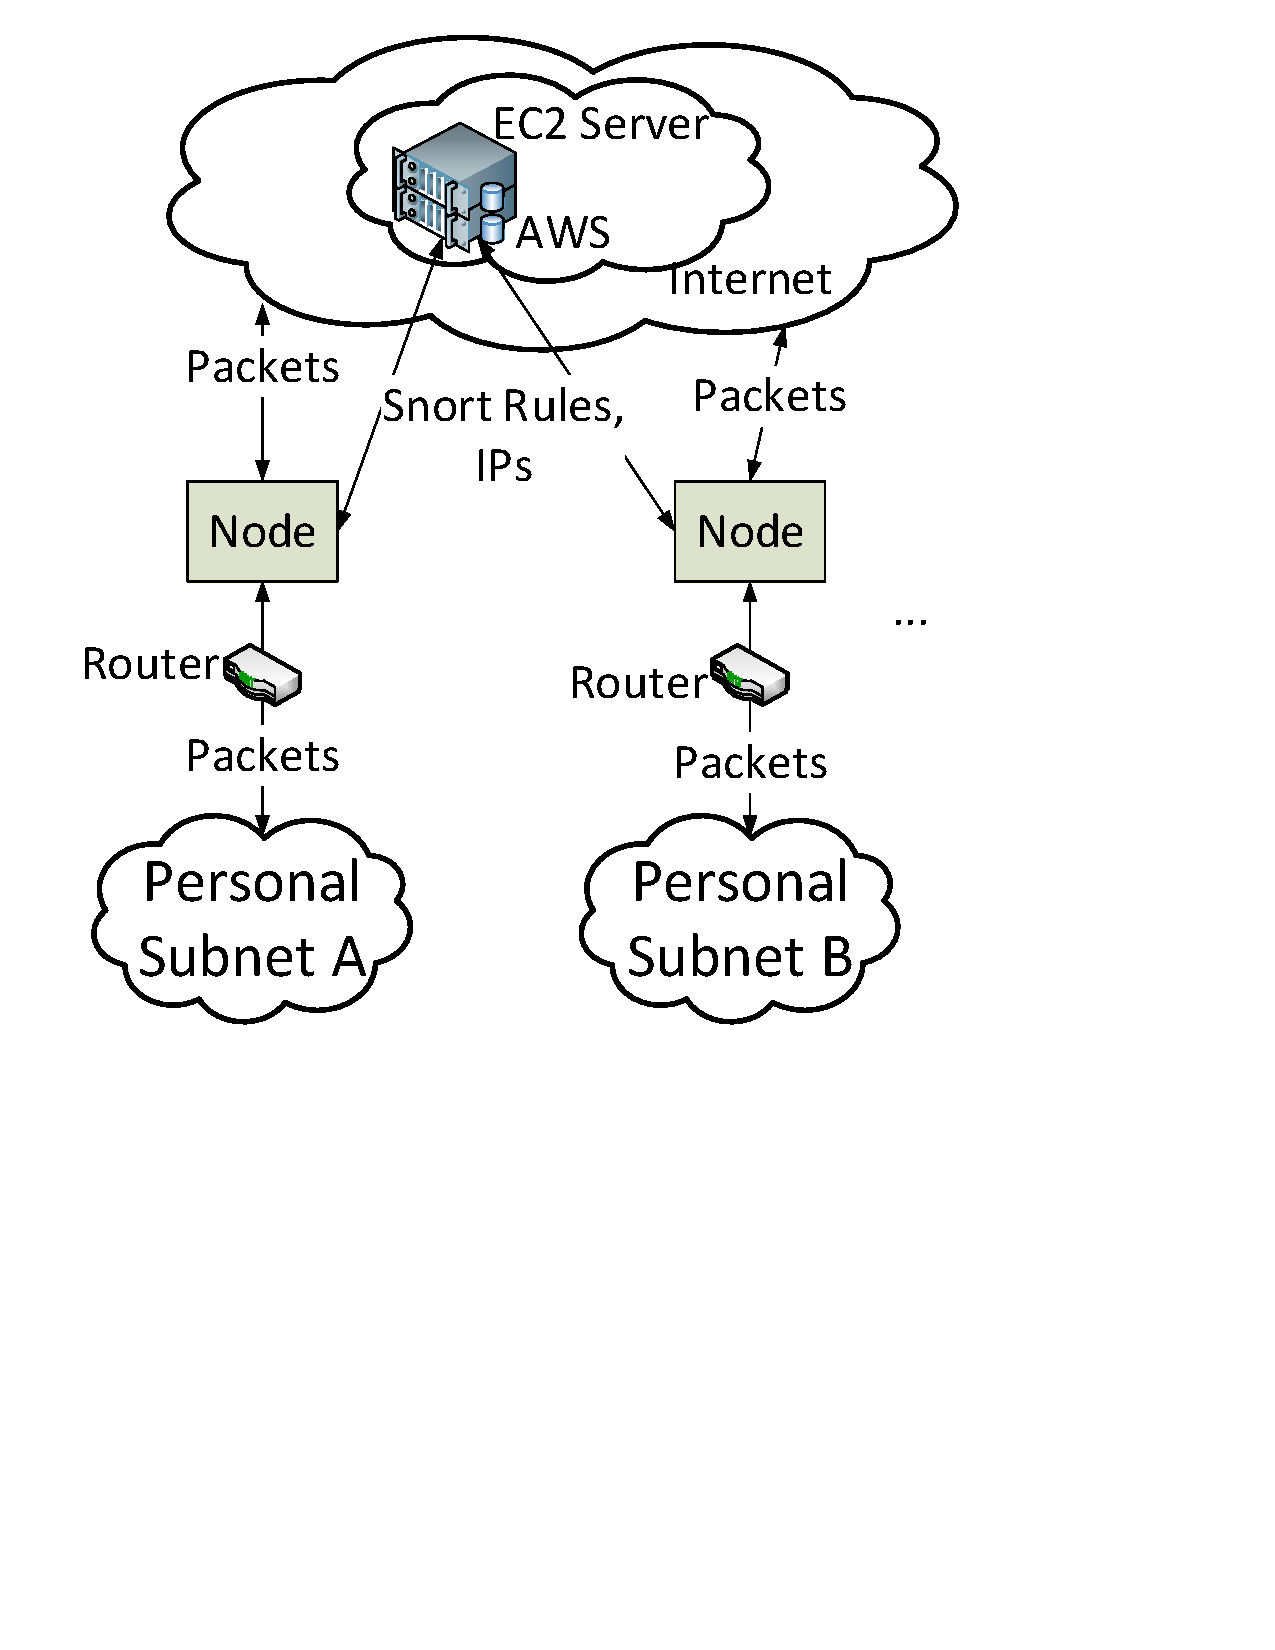
\includegraphics[height=4.4cm]{figs/macroarch.pdf}
    \caption{\sysname macro-level architecture}
    \label{fig:macro}
\end{figure}



Based on these factors, the ideal placement of the \nodename is between a Modem and Router. For networks using a Modem and a Router on the same device, we foresee that a production scale implementation of \sysname would place the \nodename hardware within the same box as the Modem and the Router, therefore maintaining the same architecture as shown in Figure~\ref{fig:macro}. Such \nodenames placed at the entry point of home networks can create a solid net of protection that can communicate threats as soon as they emerge. It must be noted that the capability of \sysname in deterring threats (and especially its ability to stop DDoS attacks) is proportional to the amount of subnets that use a \nodename; ideally there would be a \nodename within every household and business subnet.

\subsection{\nodename}
\label{sec:design:guardian}

\subsubsection{Hardware Design}
The BeagleBone Black, a reasonably powerful embedded device, was chosen as the \nodename since it satisfied the minimum requirements to implement the envisioned end product. The on-board 10/100 Mbps Ethernet port provided one network interface, while another interface was added using an USB to 10/100 Mbps Ethernet adapter. This prototype is deemed sufficient to display the core mechanics of the \nodename. 

\subsubsection{Software Design}
\label{sec:design:software}

The software design of a \nodename is depicted in Figure~\ref{fig:guardian}. The device has a DHCP server configured so that a Router can be added behind it. It passes all traffic from one network interface to the other. The \nodename runs Snort \cite{Roesch:1999:SLI:1039834.1039864}, a powerful Intrusion Detection/Prevent tool, to monitor traffic at both interfaces. A set of Snort rules are configured to block any suspicious traffic that satisfies any of the rules. Snort can perform protocol analysis, content searching/matching, and can be used to detect a variety of attacks and probes, such as buffer overflow, stealth port scans, CGI attacks, SMB probes, OS fingerprinting attempts, and many more. It also provides a black-list and white-list functionality that can be used to conditionally block and unblock malicious IP addresses. Snort was chosen as the IPS due to its large amount of documentation, open source software and up-to-date rule-lists, and its high regard in security communities. \\

Communication of malware alerts between various \nodenames is a key aspect of \sysname. This communication is done on a periodic basis by a set of three cron jobs running on the \nodename. These cron jobs do the following:

\begin{itemize}
    \item Keep Snort's general rules up-to-date by pulling rules and IPs from rule repositories.
    \item Push this particular guardian node's suspicious traffic to the \servname and also to pull new rules and blocked IPs from the \servname.
    \item Check for DDoS server beacons and generate new anti-DDoS rules if necessary.
\end{itemize}

The first cron job runs periodically and reads a log created by Snort that contains IP address of sources that have sent bad traffic. It then parses the source IP addresses present in the log, and updates the same to the database on the \servname (described in the following section). \\

\begin{figure}
    \centering
    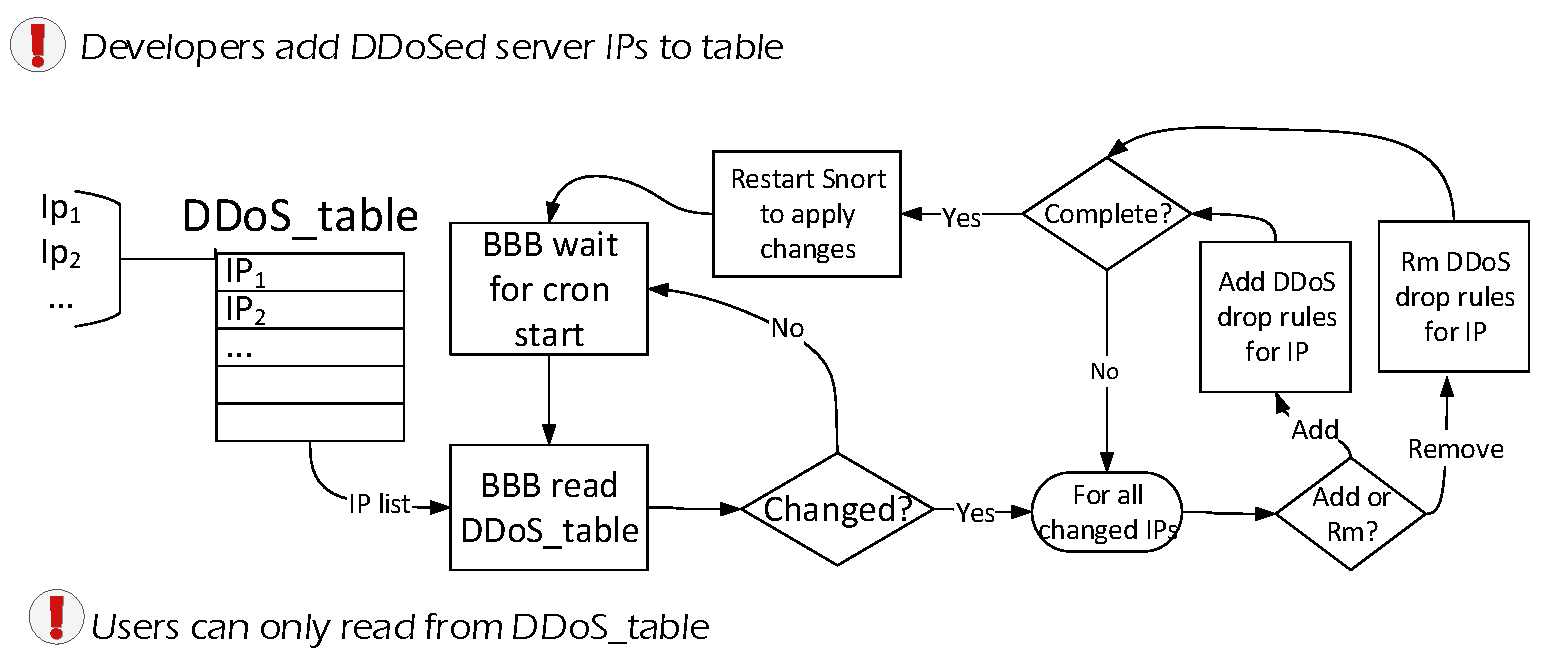
\includegraphics[width=0.95\linewidth]{figs/ddosserv.pdf}
    \caption{Outbound DDoS prevention Algorithm}
    \label{fig:ddostable}
\end{figure}

\begin{figure}
    \centering
    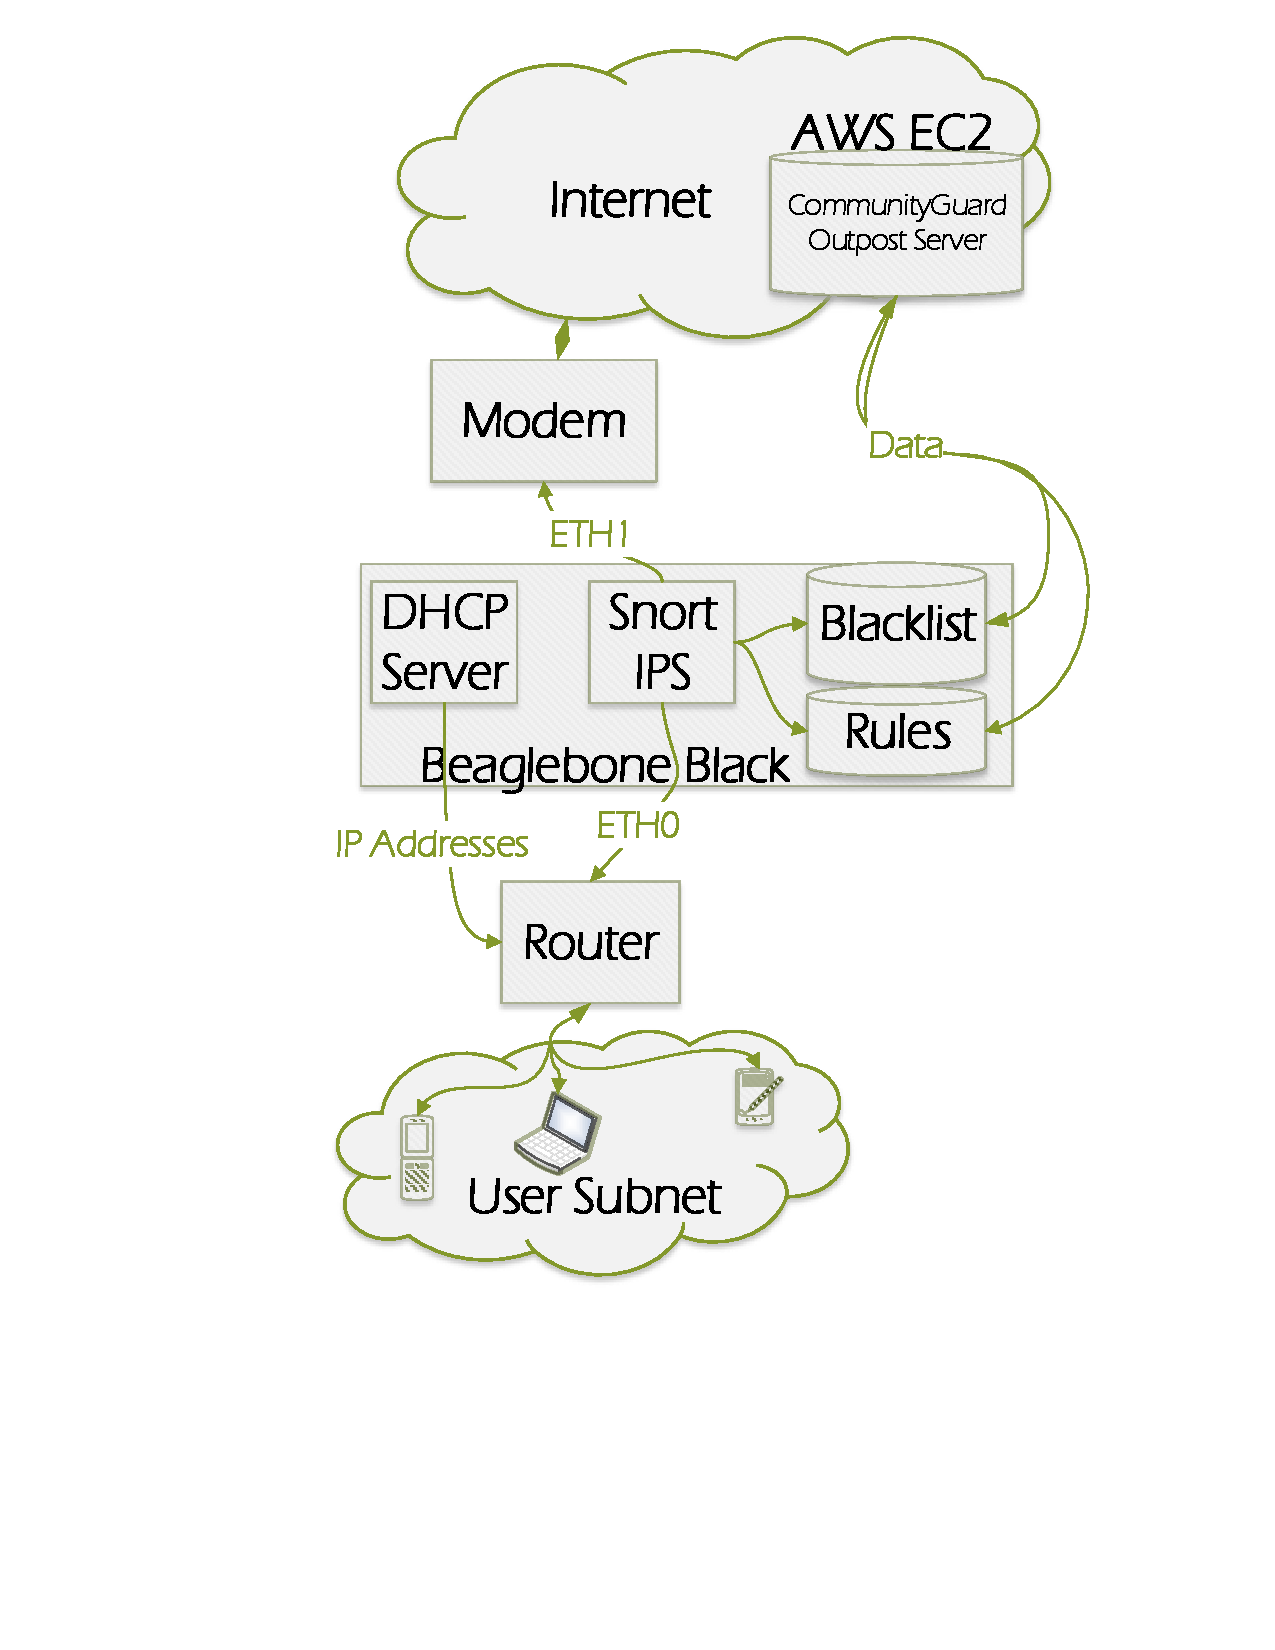
\includegraphics[height=5.5cm]{figs/microarch.pdf}
    \caption{Anatomy of a \servname}
    \label{fig:guardian}
\end{figure}

A second cron job runs periodically to fetch information from a DDoS watch list available on the \servname described below as part of the Outgoing DDoS prevention mechanism (server-side is described in Section \ref{sec:design:serverddos}). If the database provides new IP addresses (for which rules do not exist on the \nodename yet) that are currently being DDoSed, the cron job creates and adds Snort rules to drop all such outgoing DDoS traffic, thus clipping off the attack at the compromised source itself. 
This algorithm is depicted in Figure ~\ref{fig:ddostable}; Such a mechanism, when repeated over all \servnames, can prevent a DDoS attack from the source. \\

Finally, the third cron job runs once every day at some random time and fetches the latest bad IP list from the \servname and adds it to the Snort IP Blacklist. It also fetches Snort rules from Emerging Threats ~\cite{emerging} to defend against new and emerging attack patterns. These three cron jobs, combined with Snort running on all \nodenames, together establish a system of protection that learns, communicates, and has the capacity to prevent most malware attacks.

\subsection{\servname}
\label{sec:design:server}

% TODO I know I need to crop this
\begin{figure}
    \centering
    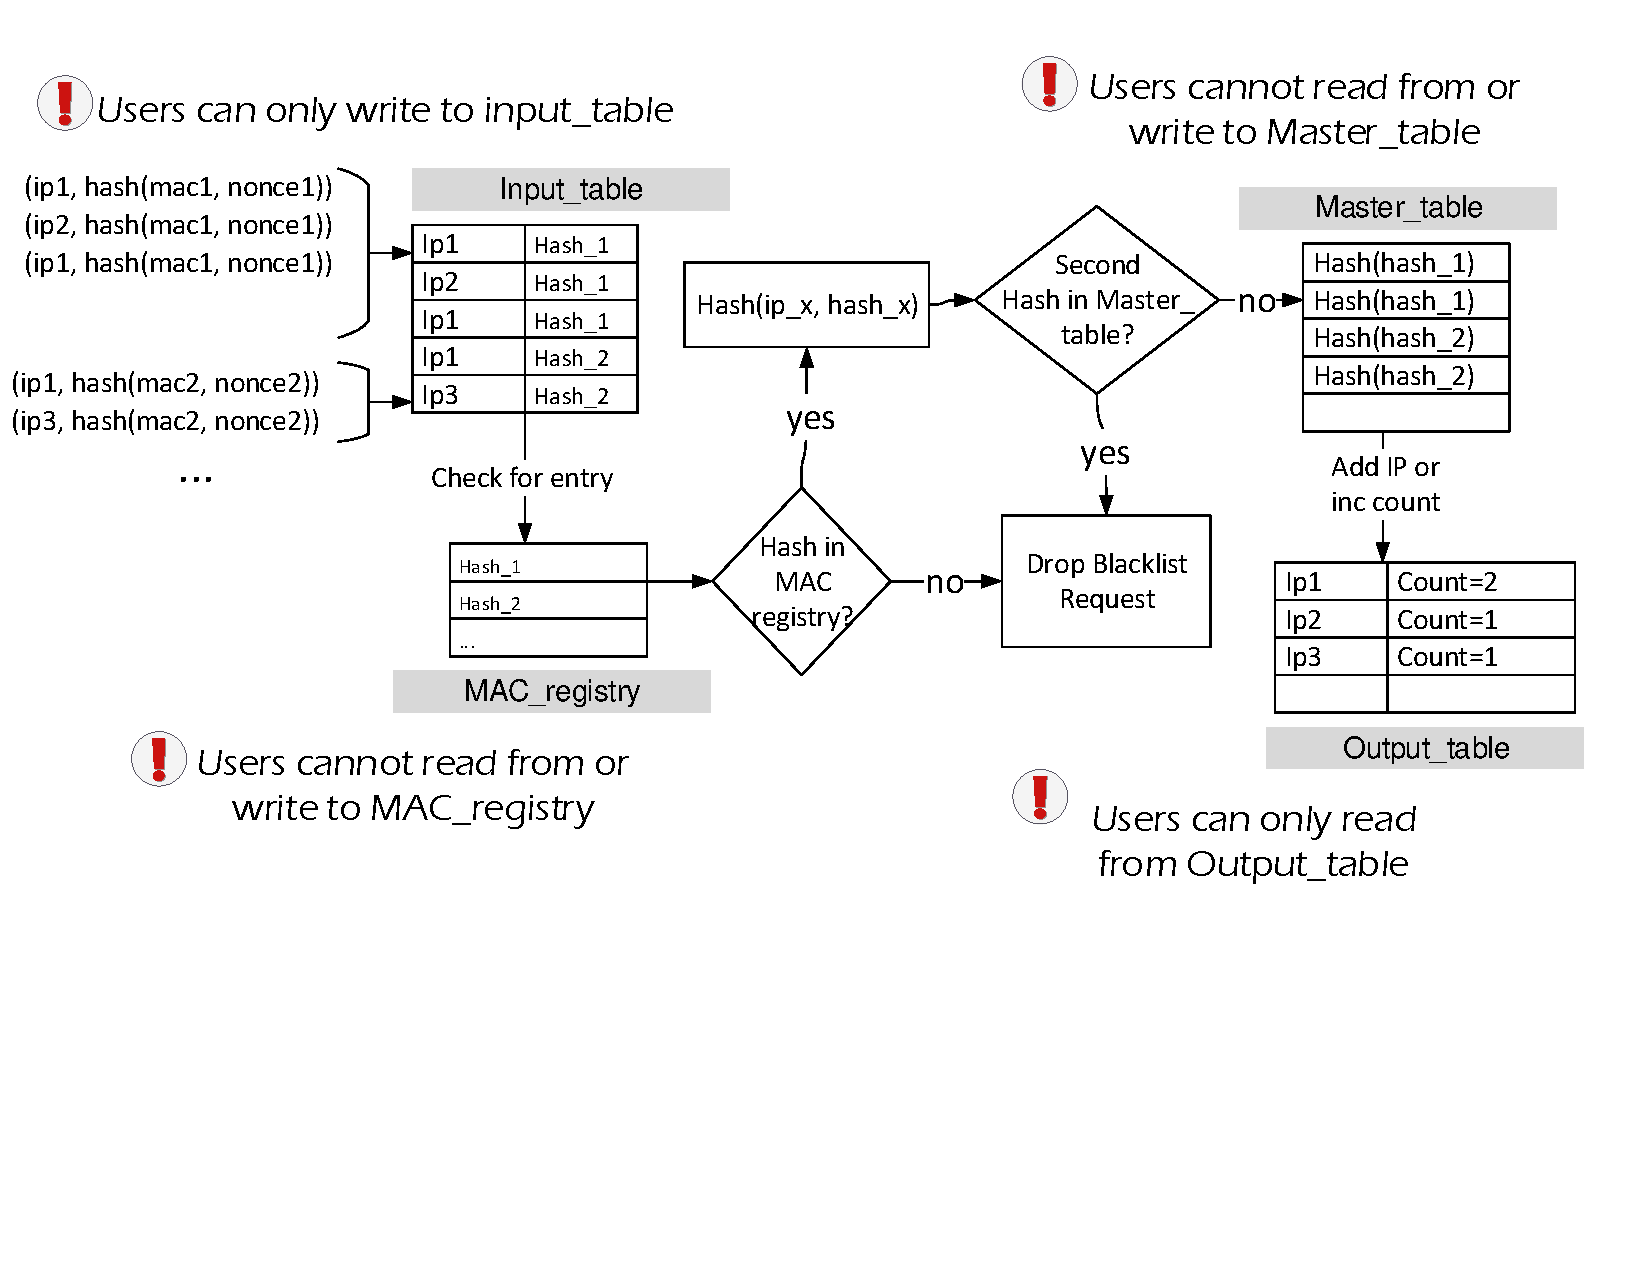
\includegraphics[width=0.95\linewidth]{figs/blacklist.pdf}
    \caption{\servname push and pull }
    \label{fig:blacklistserver}
\end{figure}

The \servname is the source of intelligence for the \nodenames that it services. This server runs a database and a couple of cron job timed events to process the information within its database. This server uses its database tables to aggregate threats presented by all collected guardian nodes, process them to determine valid threats, and then present them for individual guardian nodes to read and process. As this server is an obvious target for one who would wish to halt the \sysname service, it is foreseen that the server will be elastically-scaling and secure in a production level implementation. 

\subsubsection{Attack Models}
\label{sec:design:attacks}
We assume that a user will not attempt to attack or compromise the availability or function own \nodename since our system aims to protect users who are unaware that their devices have been compromised. Furthermore, the \nodename itself can be fortified from external attacks through a hardened OS image and security best practices. This leaves a malicious user two possible vectors of attack for causing harm to a particular user- either attempting to get harmful traffic through the \nodename, or else reverse-engineering the \nodename to attack the \servname itself. 
We designed the functionality of the \servname while keeping the following attack models in mind:

A malicious user may attempt to:
\begin{enumerate}
\item add useful IPs to the blacklist to block them for users
\item remove blacklisted IPs from the blacklist
\item read user data from the list
\end{enumerate}

\subsubsection{Server Blacklist architecture}
\label{sec:design:blacklist}
When any guardian node is created, a SHA256 hash of the node's MAC address and a random nonce stored on the \nodename's memory is entered into the mac_addr_registry table, as shown in Figure ~\ref{fig:blacklistserver}. This hash value will serve as a key for writes, to ensure that writes can only be initiated from a valid \nodename.

The \nodename is only allowed write permission to the IPv4_input table and read permission from the IPv4_output table and DDoS_output table. This policy prevents attack models 1, 2, and 3 and ensures that even if a malicious user were to reverse-engineer the device to discover a means to contact the \servname directly, the amount of damage they could cause is minor. When a \nodename is scheduled to push suspicious traffic to the \servname, it is allowed to write only into the IPv4_input table. It will write the following pair to the input table: \[\{ip_{suspicious}, SHA256(int(MAC addr), nonce)\}\] 

The \servname will process the input table to recalculate new threats at a certain frequency, and then drop the current input table. For each entry in the input table, the server first checks the SHA256 passed by the \nodename to ensure that this key is already within the mac_addr_registry. The entries that do not have a valid SHA256 hash are dropped, leaving only the valid requests. For all valid requests, a second SHA256 hash is computed, this time a hash of both the previous SHA256 result and now also the IP address declared as suspicious \[SHA256(\{ip_{suspicious}, SHA256(int(MAC addr), nonce)\}) \]. The \servname checks whether this hash is already in the IPv4_master_list server, which is a list of the SHA256, IP combinations that have previously been entered- if this is a new suspicious IP, or it is a known suspicious IP being reported by a new and valid \nodename, it will be pushed to the IPv4_output table. This second hash function ensures that a given \servname receives only one vote towards a given IP address, as a means to prevent against attack model 1. 

If this IP is a new entry, it will be entered into the table with a count of 1; if it already exists within the table, its count will be incremented. Once the count tallied against the IP reaches a sufficiently high number proportional to the number of reported threats, the IP will be pushed as output to requesting \nodenames, and blocked automatically by all \nodenames. Relying on a count before pushing a suspicious IP also helps prevent attack model 1 from occurring. 

\subsubsection{Server Outgoing DDoS prevention}
\label{sec:design:serverddos}

As mentioned above in Section ~\ref{sec:design:software}, the \servname also provides a method to prevent outgoing DDoS traffic from a \nodename's subnet out to a DDoS target. This system is much more simple than the blacklist method described above: in this case, the DDoS victim list will be edited by \sysname administrators, and only reading will be allowed for all \nodenames. \sysname administrators will confirm the existence of a DDoS attack through an alternate channel, possibly a third party DDoS \cite{DDoSPreventionTools} working with \sysname administrators, and then add the relevant IPs or CIDR ranges to the IPv4_ddos table. \nodenames will use the cron described above to add and remove rules to prevent outgoing DDoS attacks.